\documentclass[]{article}
\usepackage{hyperref}
\usepackage{graphicx}
\usepackage{wrapfig}
\usepackage{caption}
\usepackage{indentfirst}
\usepackage{subcaption}
\graphicspath{ {images/} }

%opening
\title{BattleLog: Leveraging ProbLog\\
	to Play Battleship}
\author{Noah Hadfield-Menell and Timothy Portfolio}
\date{\vspace{-5ex}}
\begin{document}

\maketitle
\begin{center}
	\url{https://github.com/nhadfieldmenell/BattleshipSRL}
\end{center}

\begin{abstract}
	
The objective of this project was to create an algorithm that can solve Battleship games more efficiently than alternative existing algorithms. The main improvement presented in this paper is the utilization of relational information that can be extracted from any board state. To accomplish this, a framework dependent on ProbLog, a probabilistic version of Prolog, was used. Comparisons of BattleLog against other algorithms demonstrate improvement in the number of moves needed to solve boards of arbitrary size and with random boat selections. 
	
\end{abstract}

\section{Introduction}

The original game of Battleship and modifications made for BattleLog are explained in this section. 

\subsection{Standard Gameplay}
\vspace{-2ex}
\begin{wrapfigure}{r}{0.40\textwidth}
	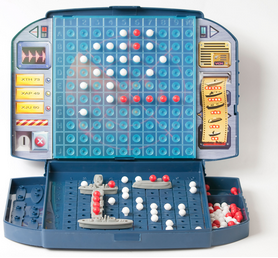
\includegraphics[width=5cm, height=5cm]{battleship}
	\captionsetup{justification=centering,margin=0.25cm}
	\caption{The physical board game representation of Battleship.}
\end{wrapfigure}

In the original game of Battleship, there are two players who play head-to-head. Each player places five boats of sizes 2, 3, 3, 4, and 5, respectively, on a square grid of 10 units in each dimension. The general setup can be seen in Figure 1. 

The players take turns, calling out a space on their opponent's grid to "take a shot" at that position. The opposing player responds with an indication of whether the shot has hit a boat or missed; the player must also indicate the length of a boat that is sunk by a hit, which means all positions of that particular boat have been called. The game ends when one player's entire fleet of boats has been sunk.

\subsection{Adjustments for BattleLog}

For the purpose of BattleLog's implementation, the game of Battleship is no longer restricted to the specific boats and grid size aforementioned in the previous subsection. Instead, the game is able to be played with an arbitrary number of boats of particular lengths on an arbitrary square grid size (e.g., a 6x6 board with three boats of lengths 3, 3, and 4). This allows for testing of various board setups for move efficiency.

Additionally, the game is not played head-to-head. Instead, the game is played by a single player (i.e., the AI) for the purpose of emphasizing the importance of move efficiency. 

\section{Implementation}

The project required the use of ProbLog for the relational approach to solving the game. Additionally, Python 2.7 served as the language of choice for the implementation of the general game framework, the comparative algorithms, the gameplay automation, and the graphical game representation. 

\subsection{Game Fundamentals}

To instantiate a game, two main classes were written: \textit{board} and \textit{game}. The \textit{board} class, given arguments for board size and boats to place on the board, creates a representation of the board with the desired constraints. It also keeps track of attributes of the board, such as the state of all positions (hit or miss) and the state of all boats (afloat or sunken).

The \textit{game} class is responsible for handling actions within the game on a move-by-move basis and tracking information about the game being played, such as the number of moves taken. Most importantly, this is where the implementations of all AI algorithms are written and utilized. 

\subsection{AI Algorithms}

The ProbLog-based algorithm as well as three other pre-existing algorithms used for playing Battleship are explained in this section.

\subsubsection{BattleLog}

The ProbLog-based AI plays the game by first generating a ProbLog script that represents a given Battleship game as a set of relationships.  This script instantiates a variable for each boat and establishes the following logic: 

\begin{itemize}
	\item Each boat must be located in exactly one canonical location, which is specified by the topmost position for a vertical boat and the leftmost position for a horizontal boat
	\item There is an equal chance that each boat is situated in each valid canonical location
	\item No two boats can occupy the same position
	\item "Hits" and "misses" are explicitly linked to boat locations
\end{itemize}

With this established, the ProbLog system can be queried for the position with the highest probability of being inhabited by adjusting the script \textit{query(boat\textunderscore in(X,Y))} for each unguessed position (X,Y) and feeding the script into a call of ProbLog's \textit{evaluate()} method.  The ProbLog system then generates a PSDD (probabilistic sentential decision diagram) that represents the game and returns the queried board positions with their associated membership probabilities. With these pieces in place, the AI plays the game by repeatedly iterating over the following steps until all boats have been sunk:

\begin{enumerate}
	\item Query the ProbLog system for all unguessed board positions.
	\item Shoot at the board position that has the highest probability of containing a boat.
	\item Add new knowledge to the ProbLog script.
\end{enumerate}

The new knowledge that the AI adds to the ProbLog script at the end of every turn is related to the feedback from the \textit{game} class after it records a shot.  For a hit or miss, the AI records as evidence that there is (or is not) a boat in the queried position. In the presence of a sink of a boat of length Z, the AI adds all knowledge that can be inferred from that outcome: namely that any consecutive collection of recorded hits that includes the guessed position and is of length Z could potentially hold a boat. More specifically, exactly one of these canonical locations is the one that describes the boat that was just sunk. Additionally, in the presence of a hit without a sink, the script asserts as evidence that none of the canonical locations that would have been completed by a hit in that position holds a boat. For example, if hits have been recorded in positions (1,1) and (1,3) and another hit is observed in (1,2) without a sink, evidence is added to the script asserting that there is no horizontal boat of length 2 located at positions (1,1) or (1,2) and that there is no horizontal boat of length 3 located at (1,1).

\subsubsection{Random}

This is the least sophisticated of the four algorithms employed. Every shot is taken at a position randomly drawn from the set of positions that have yet to be shot at. This algorithm does not take advantage of any information whatsoever that can be gained from the board state.

\subsubsection{Hunt-and-Target}

This algorithm starts by shooting randomly at positions that have yet to be tried (i.e., "hunting" for a boat). Once a hit has been detected, the four adjacent cardinal positions (i.e., north, south, east, and west) are added to a target list, as long as they have yet to be tried. The target list operates as a FIFO set of high-priority positions to shoot at. Positions can be added to the target list if more hits are accrued. When the target list is empty, the algorithm resorts to random selection of unshot positions once more.

\subsubsection{PDF}

The PDF (probability density function) algorithm is often referenced as a very strong approach to solving a Battleship game in a short number of moves. The algorithm starts in its own refined "hunt" mode, where it creates a scoring matrix for each boat that is present on the board. For each boat, it determines the number of possible orientations that pass through each position on the board. A score is then assigned to each position. A composite score is generated by combining the results of each score matrix. The algorithm selects the highest-scoring position to shoot at. For a miss in hunt mode, the algorithm will re-evaluate the board state and again calculate a composite score matrix. If a hit results, then the algorithm enters its "target" mode.

In the "target" mode, possible boat orientations that pass through multiple hit positions yet to be attributed to a sunken ship receive a much higher weight. This allows for a quicker removal process of partially hit boats. Once a boat is sunk and no leftover hits remain, the algorithm resumes its "hunt" mode, but it only performs calculations using boats that are known to be still in play.

A couple of notable weaknesses are present in this algorithm relative to the ProbLog-based one. One is that the PDF algorithm struggles with ambiguity of the location of a sunk boat if multiple boats are revealed to be adjacent to one another. Additionally, the PDF algorithm considers all boats on the board as independent entities when hunting; for example, it ignores that boats cannot overlap when it comes to creating score matrices.

\subsection{Gameplay Automation}

In order to gather data on the performances of the algorithms mentioned above, an automation system was implemented. Before the entire system was created, however, several changes to the underlying \textit{game} class were necessary. One of the most important changes was the modification of the Python framework that manages games running the ProbLog algorithm. As the ProbLog method uses significant amounts of memory to perform board state evaluations, it became necessary to force garbage collection after each move via subprocess instantiation to allow for consecutive games to be run in one call. Additionally, intermediate game state data had to be pickled and re-introduced into the main instance to preserve game integrity. 

The automation system utilizes a multi-layered folder structure that separates data files first based on the game type (e.g., a game played with the random algorithm, a board of size 7, and three boats of sizes 5, 5, and 4). The naming convention is ALGORITHM\textunderscore BOARD-SIZE\textunderscore BOAT-1\textunderscore...\textunderscore BOAT-N. The example provided in this paragraph would appear as RANDOM\textunderscore 7\textunderscore 5\textunderscore 5\textunderscore 4.

The subfolders are named by the UNIX time of the operation. In each of these subfolders, information about each game iteration (e.g., number of moves and time to completion) is written to a file \textit{runX.data}, where X is the zeroth-indexed game iteration. An additional file, \textit{summary.data}, tracks composite and average information based on the individual runs. 

\subsection{Graphics}

The Pygame library was used to create a graphical representation of a Battleship game, updating the view of the board as each move is played out. Blue tiles indicate unexplored positions, red tiles hits, and gray tiles misses. A sample for each algorithm on the same game can be seen in Figure 2. 

\begin{figure}
	\centering
	\begin{subfigure}[b]{0.475\textwidth}
		\centering
		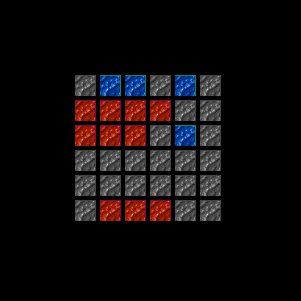
\includegraphics[width=4cm, height=4cm]{random}
		\captionsetup{justification=centering,margin=0.25cm}
		\caption{Random}
	\end{subfigure}
	\begin{subfigure}[b]{0.475\textwidth}
		\centering
		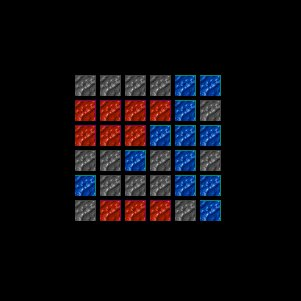
\includegraphics[width=4cm, height=4cm]{hnt}
		\captionsetup{justification=centering,margin=0.25cm}
		\caption{Hunt-and-target}
	\end{subfigure}
	\vskip\baselineskip
	\begin{subfigure}[b]{0.475\textwidth}
		\centering
		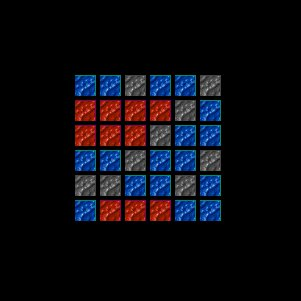
\includegraphics[width=4cm, height=4cm]{pdf}
		\captionsetup{justification=centering,margin=0.25cm}
		\caption{PDF}
	\end{subfigure}
	\begin{subfigure}[b]{0.475\textwidth}
		\centering
		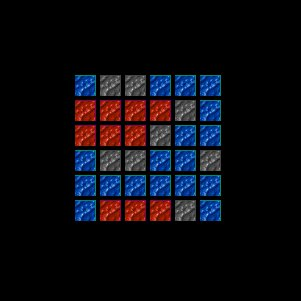
\includegraphics[width=4cm, height=4cm]{problog}
		\captionsetup{justification=centering,margin=0.25cm}
		\caption{ProbLog}
	\end{subfigure}
	\caption{Example end boards for the four algorithms}
\end{figure}

\section{Results}

In order to thoroughly test the capabilities of the ProbLog-based algorithm, a dedicated server with 144 GB of memory was used. The need for this amount of RAM is due to the combinatorial qualities of the game of Battleship when scaling the size of the grid and the number of boats in play. 

\subsection{Move Efficiency}

In less complex boards, the difference between the PDF and ProbLog algorithms in terms of move efficiency was negligible. However, the ProbLog algorithm was able to improve upon the performance of the PDF algorithm by a few moves in bigger boards. Table 1 shows the raw numbers in boards that were able to be tested across all algorithms. Figure 3 is a graphical representation of Table 1. Averages are taken over dozens of iterations of randomly generated boards with the given constraints.

%table generated with help of http://www.tablesgenerator.com/

\begin{table}[]
	\centering
	\begin{tabular}{|c|c|c|c|c|}
		\hline
		& \textbf{Random} & \textbf{HT}   & \textbf{PDF}  & \textbf{ProbLog} \\ \hline
		\textbf{4, {[}3, 2, 2{]}} & 14.8   & 13.5 & 11.2 & 11      \\ \hline
		\textbf{5, {[}3, 2{]}}    & 22.5   & 14.8 & 12.1 & 11.5    \\ \hline
		\textbf{5, {[}3, 3, 2{]}} & 22.5   & 18.9 & 14.3 & 14.5    \\ \hline
		\textbf{6, {[}4, 3, 3{]}} & 33.2   & 25   & 18.4 & 16.4    \\ \hline
		\textbf{6, {[}5, 5, 4{]}} & 34.5   & 28   & 20.6 & 19.3    \\ \hline
		\textbf{7, {[}5, 5, 4{]}} & 46.8   & 34.3 & 22.4 & 19.6    \\ \hline
	\end{tabular}
	\caption{Average number of moves taken by each algorithm}
\end{table}

\begin{figure}
	\centering
	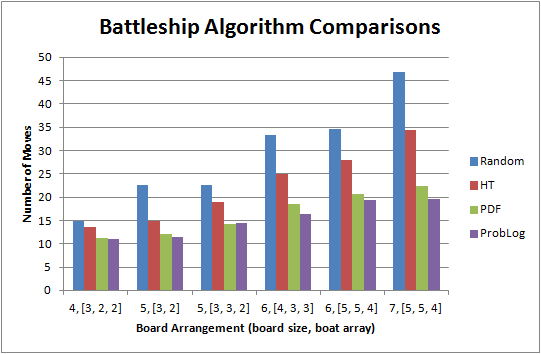
\includegraphics[width=13cm, height=8.5cm]{chart}
	\captionsetup{justification=centering,margin=0.25cm}
	\caption{Graphical representation of Table 1}
\end{figure}

\subsection{Time and Space Observations}

The random, hunt-and-target, and PDF algorithms generally completed individual games in the span of milliseconds. The amount of space needed to complete the game was negligible.

However, the ProbLog version had difficulties with time and space efficiency when scaling to larger boards. With boards of size 8, the server's entire memory capacity was exhausted and still unable to complete a move. Even with boards of size 7, moves would take roughly a half hour to complete in the earlier stages of games. As such, the ProbLog algorithm has shown that while it is more efficient in moves taken for boards within its capacity, it's not quite as versatile as other algorithms in completing large games in a reasonable amount of time and space.

\section{Conclusion}

Our experiments show that there is an advantage to representing this game as a set of relationships and using probabilistic statistical relational tools to evaluate it. As the scale and complexity increased in our trials, so too did the improvement exhibited in the statistical relational approach over the greedy approaches.  Ultimately, however, complexity was also the limiting factor in what we could achieve with this model and our given resources.
Still, this project evinces that framing problems as statistical relational learning problems, even those that might not be traditionally viewed as such, can lead to a substantial performance in their evaluations.  Given the computational complexity of the tools used to solve these problems, those wishing to do so must find a proper balance in the requirements of the problems they hope to model and the systems they are using for modeling.

\end{document}
